\section{Profile Select Activity}
This section will explain the profile select activity and how it makes some of the external architecture for others to use.

The profile select activity is very simple for the user to look at \autoref{fig:profile-select-activity} and

\begin{figure}[h!]
	\centering
	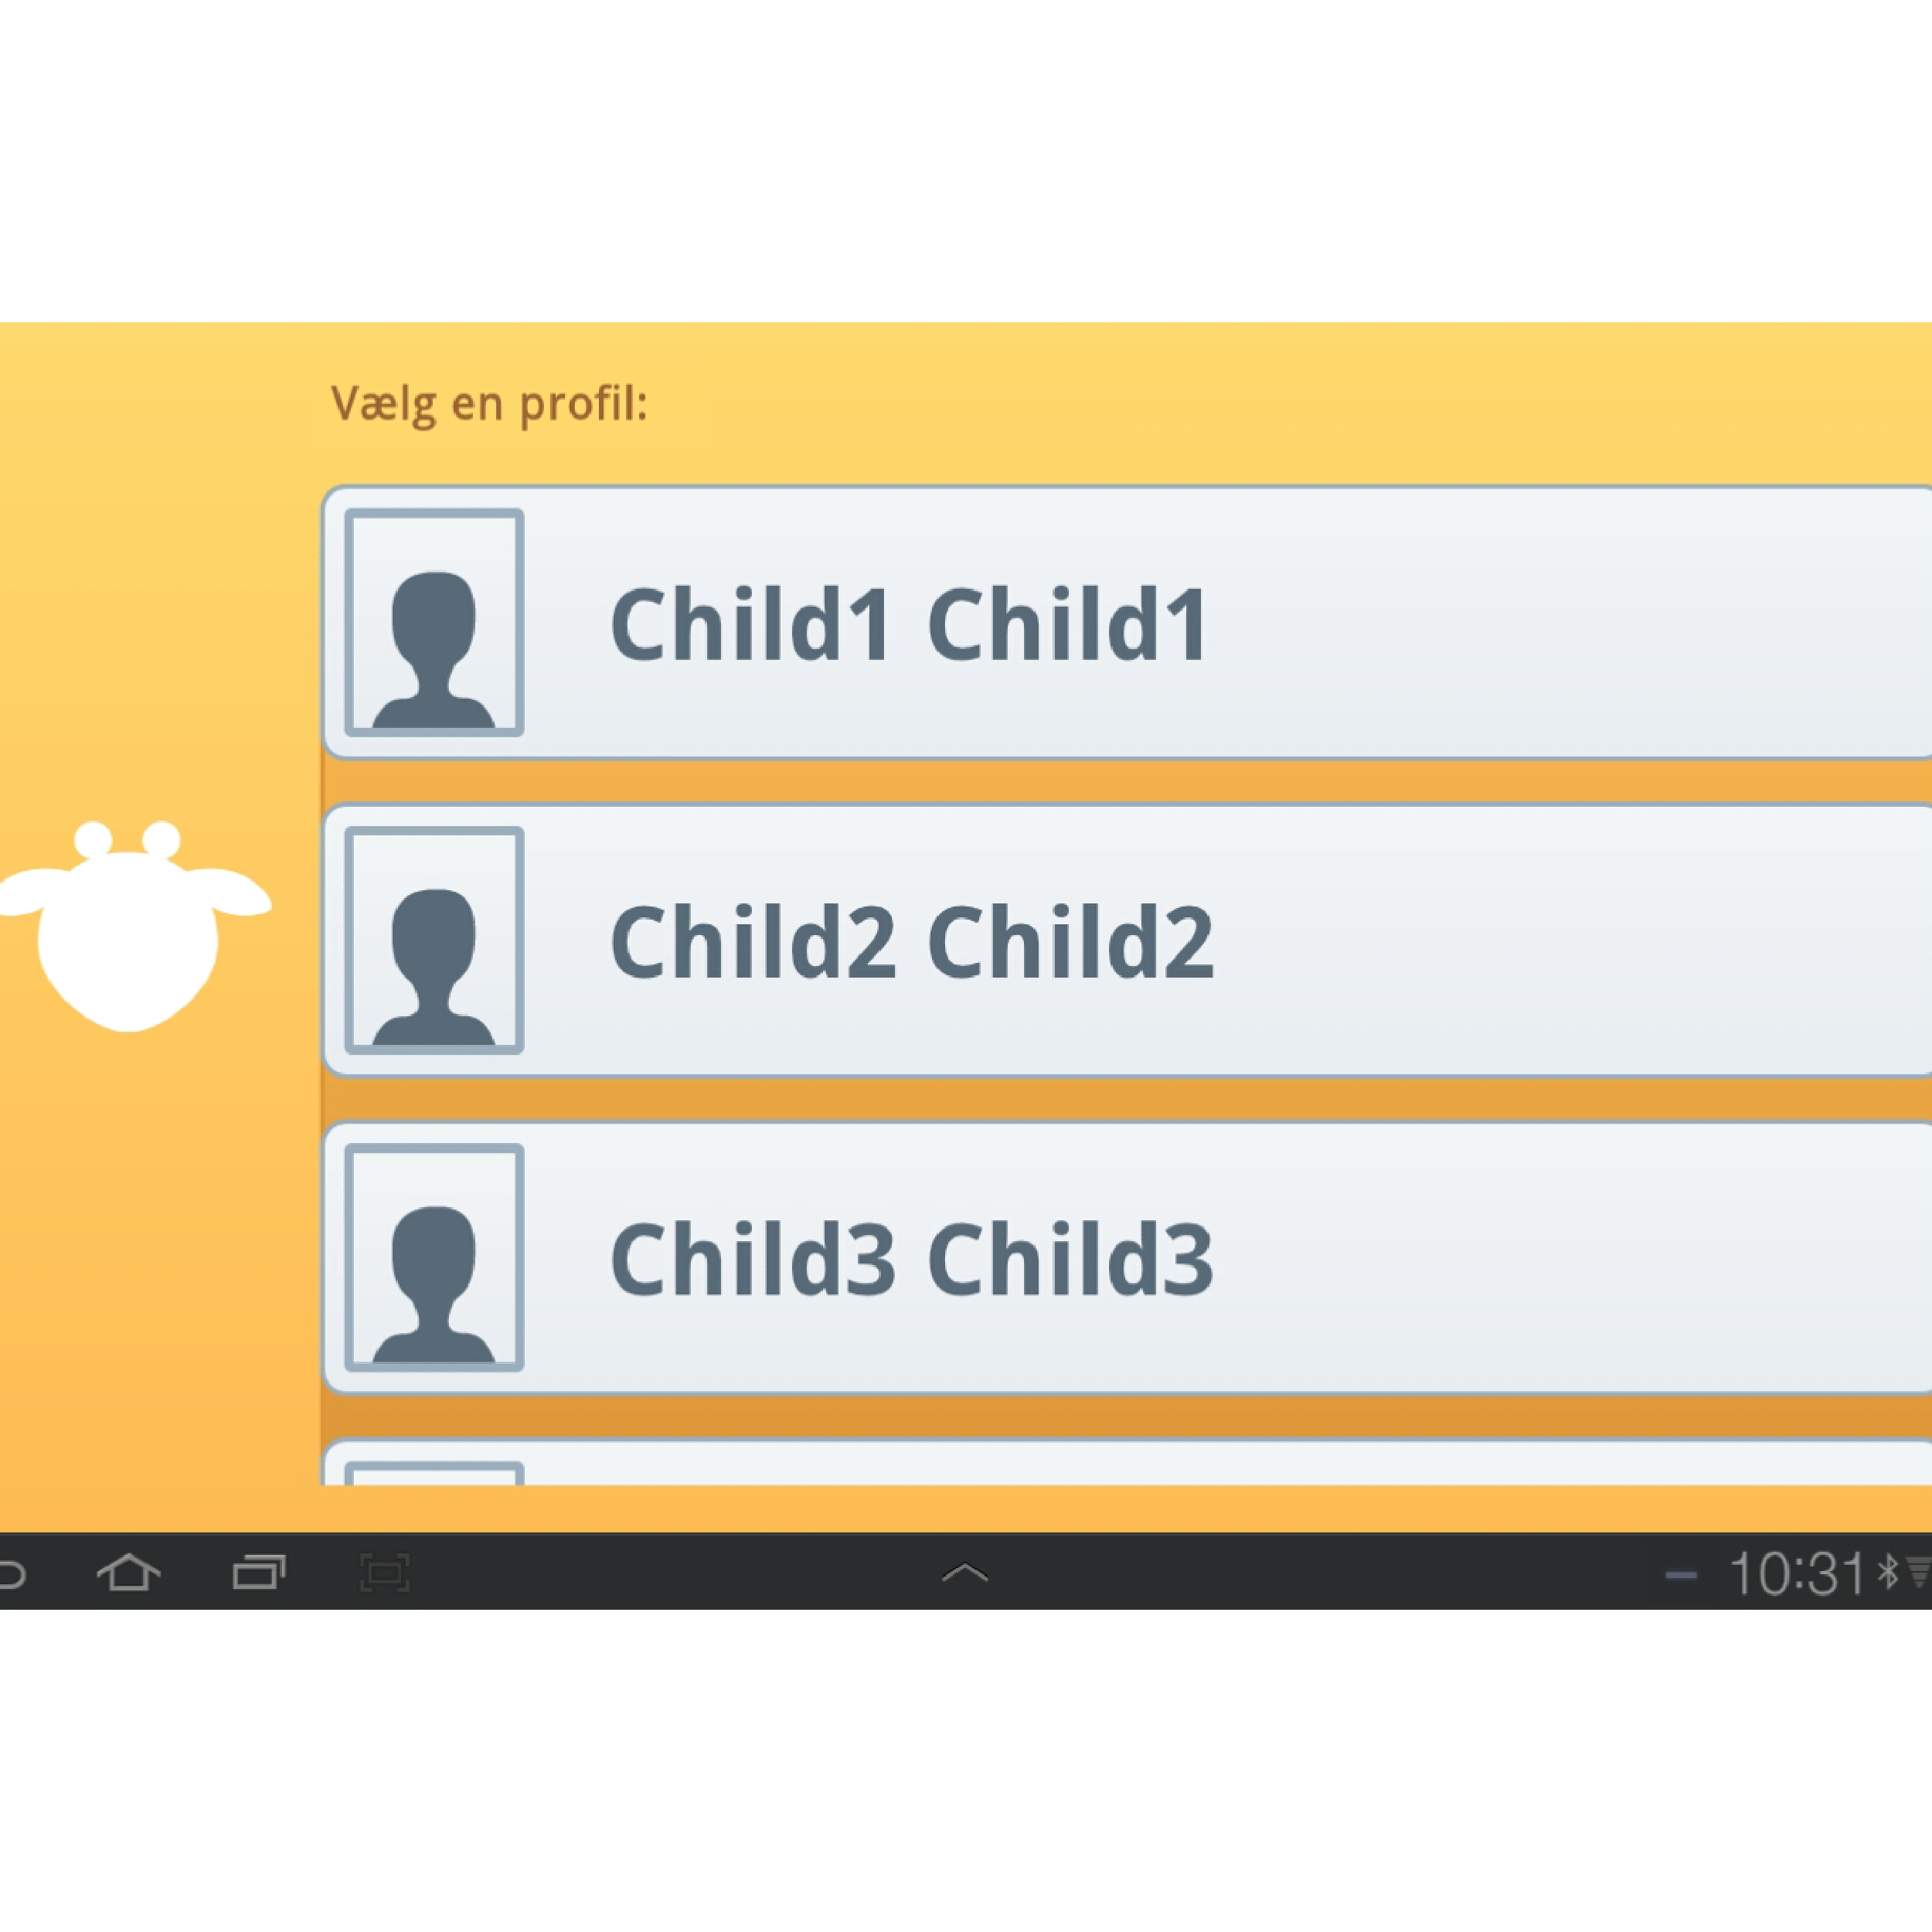
\includegraphics[scale=0.3]{gfx/profile-select-activity_2.jpg}
	\caption{Landscape profile select activity screenshot}
	\label{fig:profile-select-activity}
\end{figure}

\begin{lstlisting}[style=sourceCode, language=JAVA, caption=How the launcher shares different ids and color through the profile select activity, label=lst:profileActivity] 
listOfChildren.setOnItemClickListener(new OnItemClickListener() {
			public void onItemClick(AdapterView<?> parent, View view, int position, long id) {
				final long childID = ((Profile) parent.getAdapter().getItem(position)).getId();

				Intent intent = new Intent(Intent.ACTION_MAIN);
				intent.addCategory(Intent.CATEGORY_LAUNCHER);
				intent.setComponent(new ComponentName(mPackageName, mActivityName));
				intent.setFlags(Intent.FLAG_ACTIVITY_NEW_TASK
						| Intent.FLAG_ACTIVITY_RESET_TASK_IF_NEEDED);

				intent.putExtra(Data.CHILDID, childID);
				intent.putExtra(Data.GUARDIANID, mGuardianID);
				intent.putExtra(Data.APP_COLOR, mAppColor);

				startActivity(intent);
			}
		});
\end{lstlisting}